\section{Structure du site et style}


Pour la partie interface utilisateur, nous avons réalisé des pages web en JSP. Nous avions pour consigne de faire en sorte que celles-ci soient responsives grâce à Bootstrap. L'utilisation de scripts JSP représentaient un réel avantage dans cette tâche cas elle permettait de rendre modulable le site tout entier grâce à des liaisons avec des servlets correspondants. Chaque page, selon un lien cliquable, peut afficher un nouveau champ et modifier des éléments du Back-end. Par ailleurs, nous avons défini deux fichiers JSP, servant de header et de footer. Nous les avons appelés dans la plupart de nos pages. Grâce aux Header, il est aisé de se connecter ainsi que se déplacer à travers le site, selon l'utilisateur connecté. Le Footer, quant à lui, permet de trouver les mentions légales, un descriptif du projet et les contacts.

\begin{figure}[ht]
    \begin{center}
	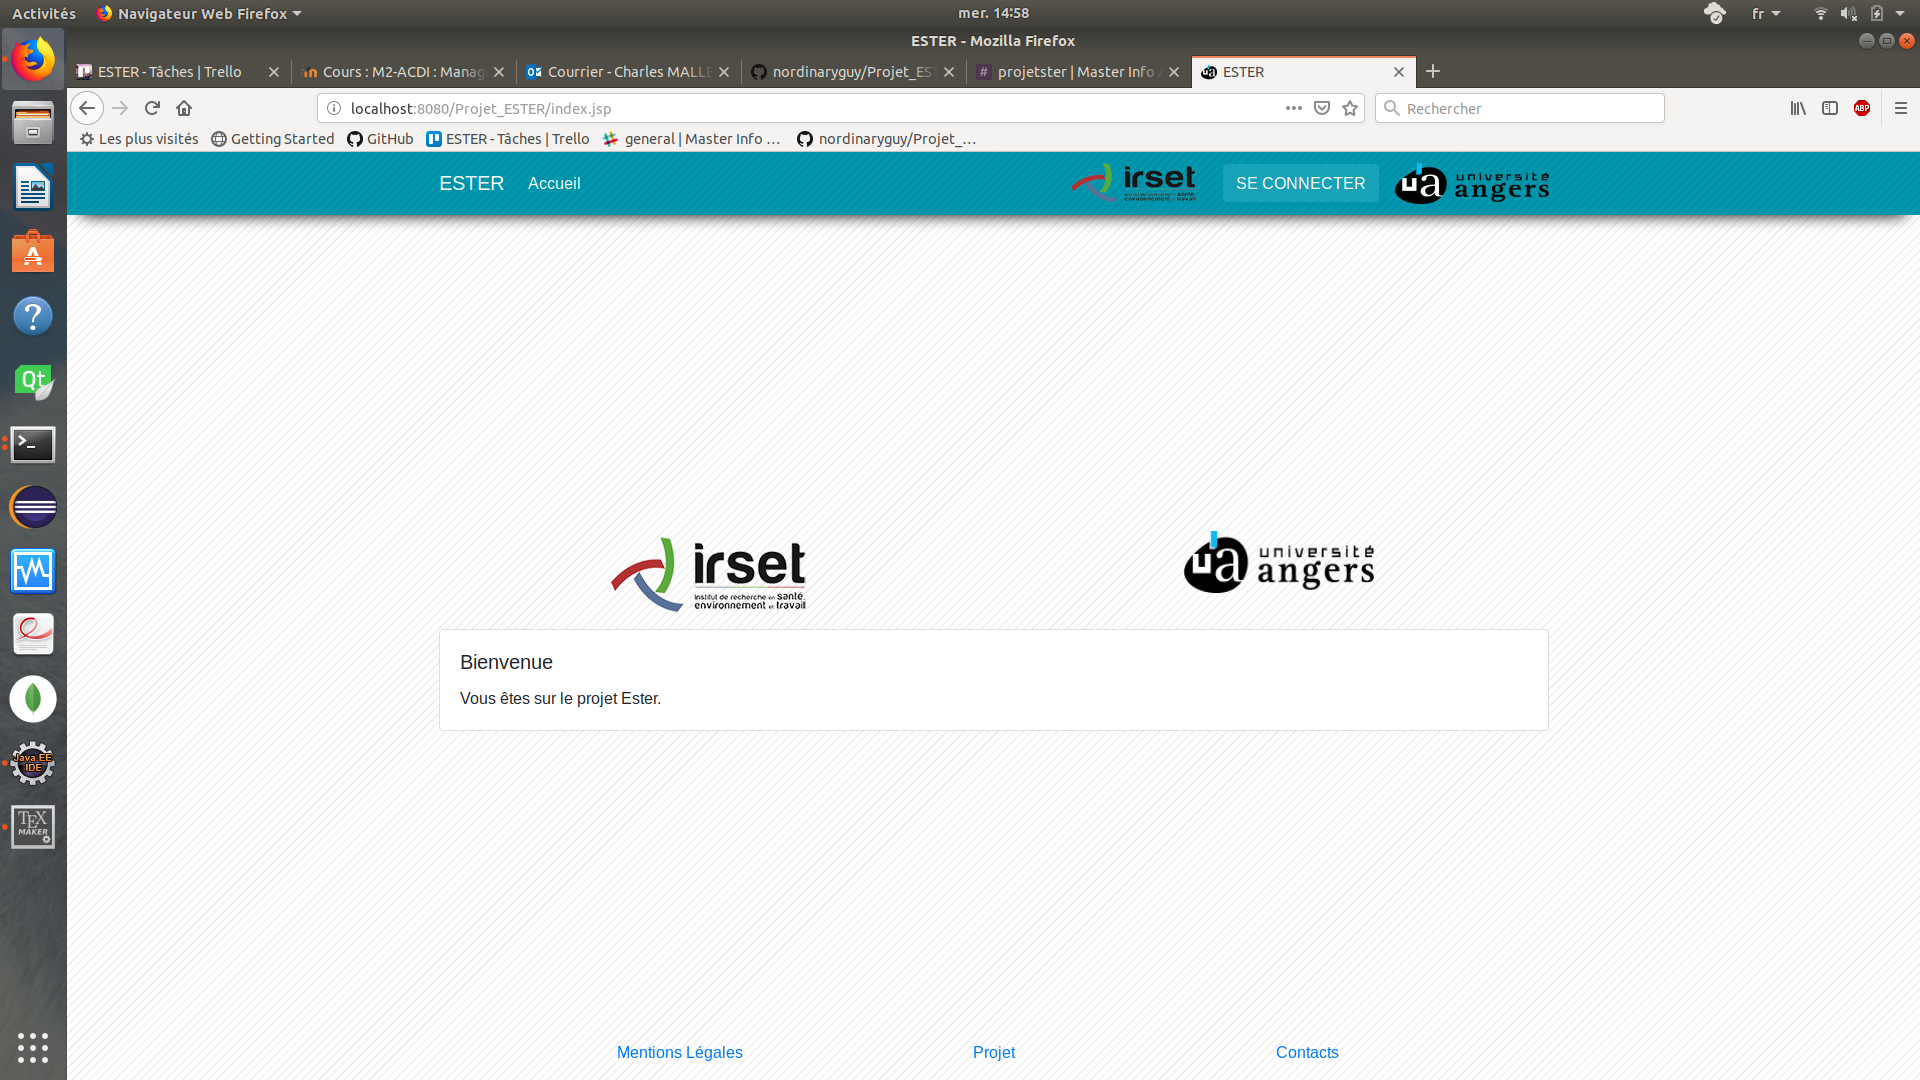
\includegraphics[scale=0.2,trim=4cm 0cm 4cm 5.3cm, clip=true]{img/ESTER}
    \end{center}
    \caption{Page d'Accueil ESTER}
\end{figure}

Afin de donner un exemple concernant l'aspect modulable de nos pages, nous pouvons regarder la page de Connexion. Sur cette dernière, en fonction du bouton sélectionné ("Salarié"/"Entreprise"/"Utilisateur" \footnote{Fait référence aux utilisateurs médicaux et aux administrateurs ; par opposition aux entreprises et salariés.}), vous aurez des champs de saisi différents. Puis, une fois la vérification effectuée, l'utilisateur du site sera redirigé automatiquement au bout de quelques secondes vers sa page.

\begin{figure}[ht]
    \begin{center}
	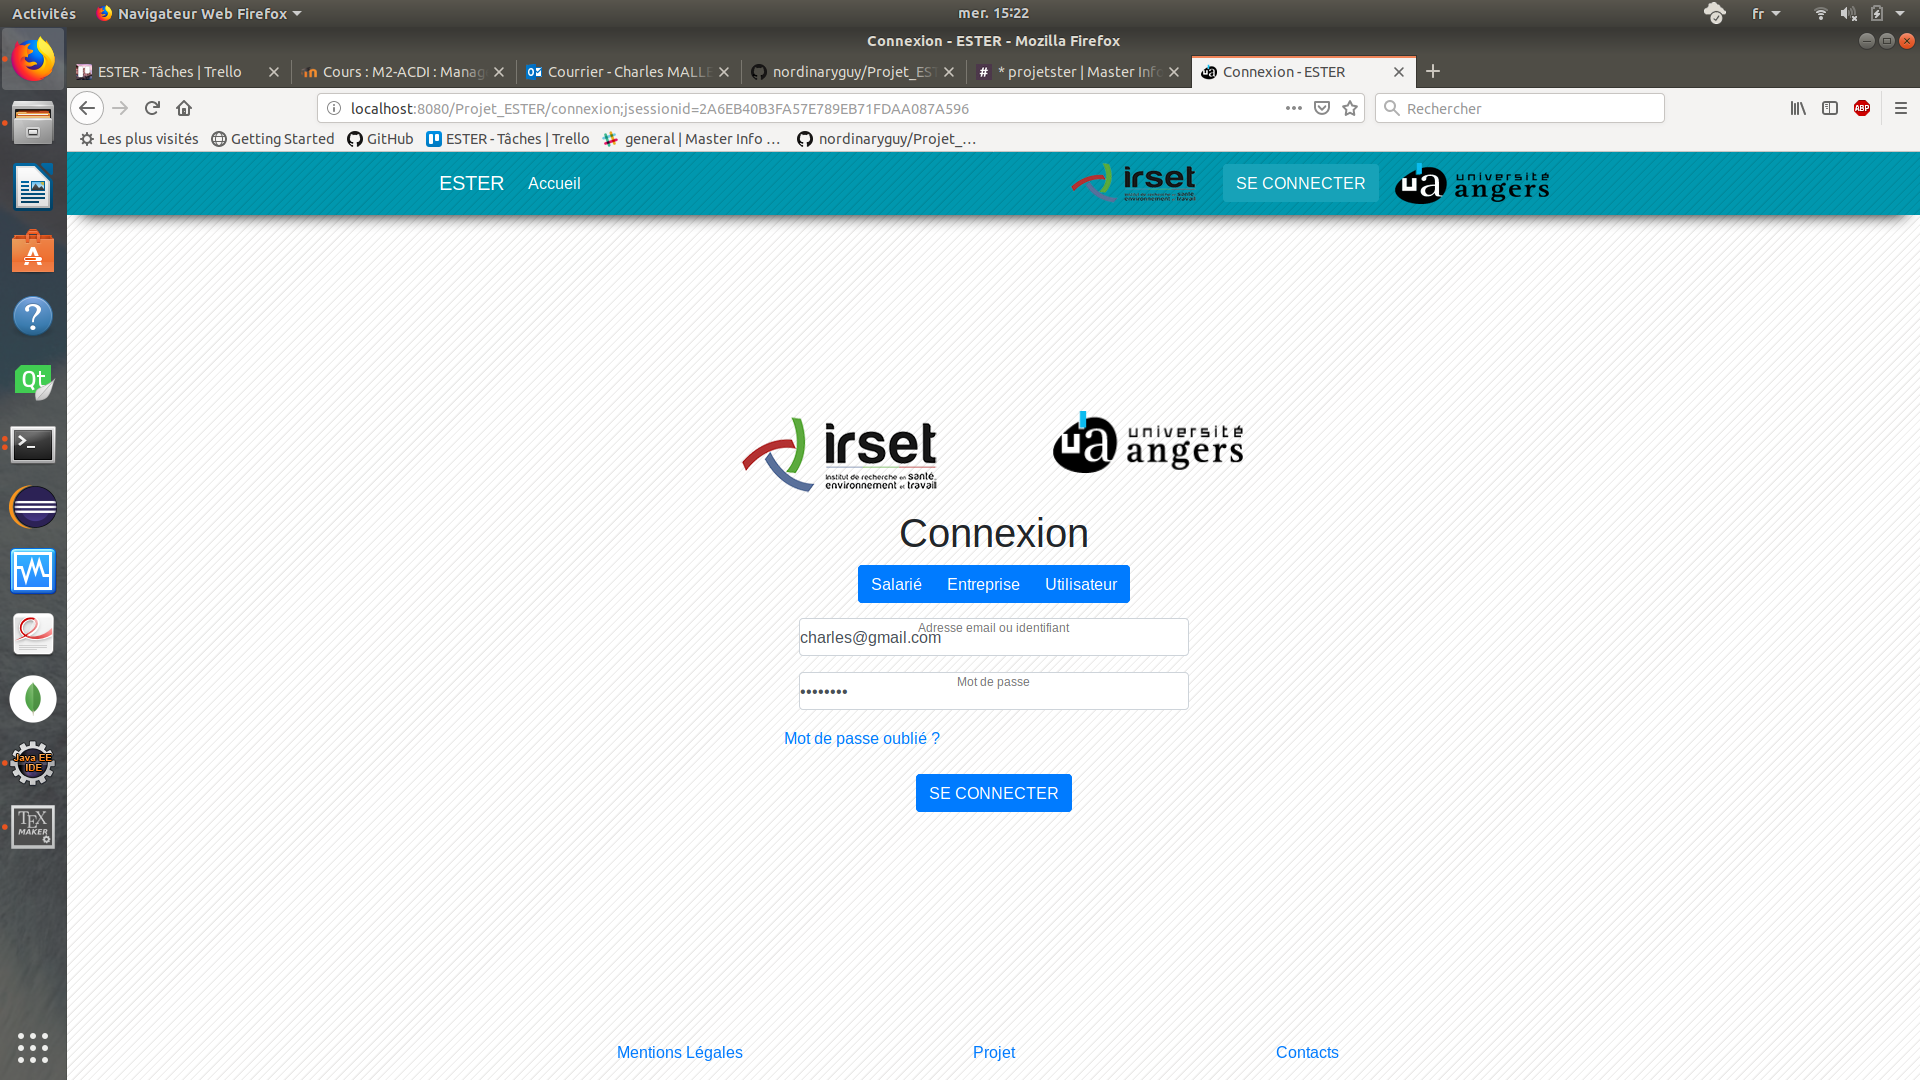
\includegraphics[scale=0.2,trim=4cm 0cm 4cm 5.3cm, clip=true]{img/Connexion}
    \end{center}
    \caption{Page de Connexion}
\end{figure}

Une fois connecté, l'utilisateur se retrouve sur la page qui correspond à son statut. Il peut choisir ce qu'il souhaite faire à l'aide des liens dans le Menu à gauche. Pour certains liens, du contenu s'ajoutera sur sa page s'il les sélectionne. Il sera également redirigé vers une nouvelle page correspondante pour d'autres. 

\begin{figure}[ht]
    \begin{center}
	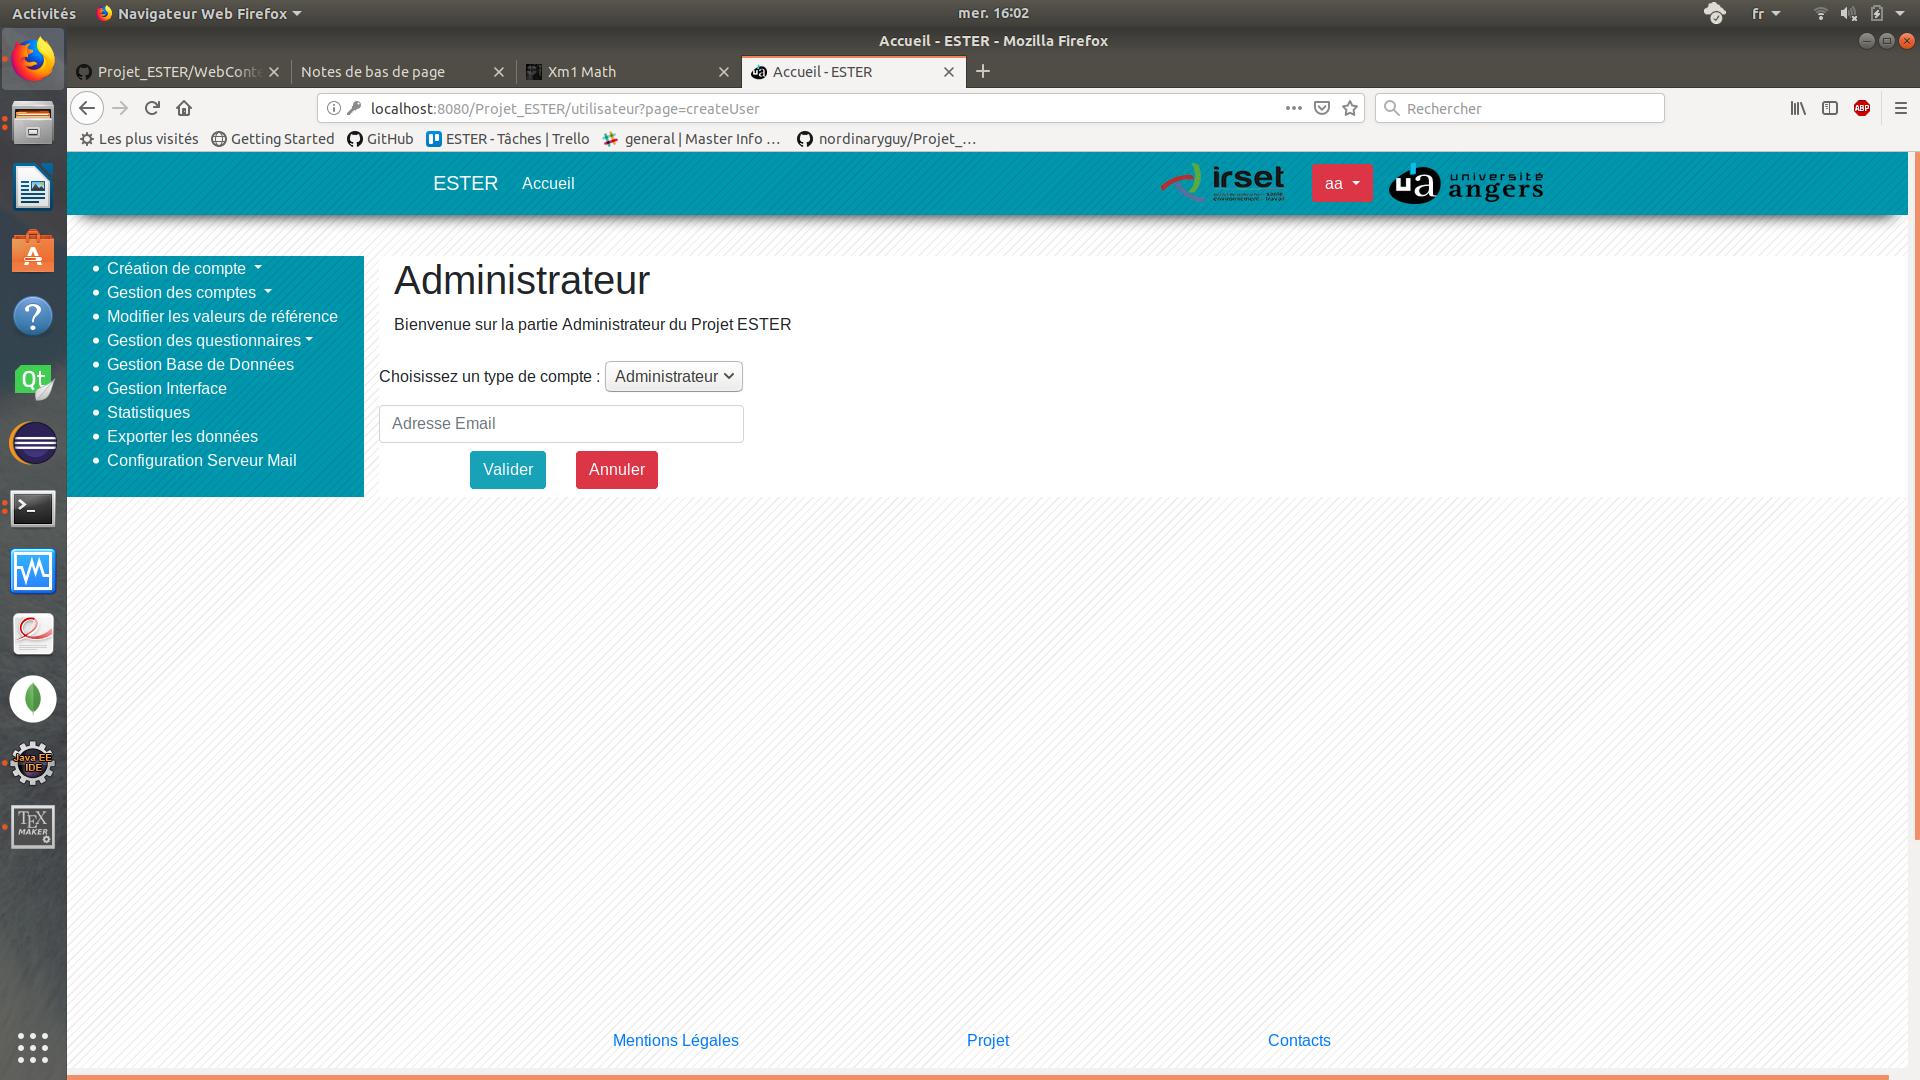
\includegraphics[scale=0.2,trim=2.8cm 0.1cm 0.8cm 5.3cm, clip=true]{img/Admin}
    \end{center}
    \caption{Page de l'Administrateur}
\end{figure}

